%%%%%%%%%%%%%%%%%%%%%%
% DESCRIPCION DEL PROBLEMA
%%%%%%%%%%%%%%%%%%%%%%

En este capítulo se describen las bases teóricas  concernientes al contexto ganadero en Colombia y el Cauca, así como también las bases teóricas de los métodos matemáticos y algoritmos computacionales aplicados a lo largo del desarrollo de este proyecto.

%En este capitulo se explica el contexto ganadero actual y algunas de las características principales relacionadas al proceso de ceba.(Esto estaba antes del 15 de Agsoto de 2019 que hice los cambios en bOSCH)

%El titulo debe ser algo como Contexto general de la ganaderia de carne

%Tengo que agregar algo como otro capitulo de solo lo del tornillo (creo que alcanza) o sino agregarlo a lo de ELECTRÜONICA EN EL AGRO y combinar ese capitulo y PONERLE OTRO NOMBRE.

\section{Contexto ganadero multipropósito} \label{contexgan}
\subsection{Generalidades agropecuarias} \label{tgan}
%\section{Visión global} \label{tgan}
%\section{Contexto ganadero en Colombia} \label{tgan}

%ESTO SE BORRA-> Explicar el CONTEXTO, síntomas y causas del problema a resolver. (1.5 páginas).EXPLICAR QUE VOY A HACER \\ \\

La fortaleza principal del sector primario colombiano radica en la producción de recursos de la naturaleza. Esto se refiere a las actividades económicas en relación a los procesos de producción en el sector agropecuario. Este sector abarca el conjunto de técnicas y las acciones que permiten trabajar y cultivar la tierra para producir materias primas así como también la producción de recursos de la ganadería. Por su parte, el sector ganadero alude a los diferentes tipos de ganado de una zona y a las actividades que se emplean para criar y comercializar a estos animales y a los productos derivados de estos. En Colombia se practican diferentes modalidades de ganadería con base en el tipo de ganado de enfoque tales como:

\begin{itemize}
\begin{multicols}{3}
    \item Bovinos ó Vacunos
    \item Mulares y asnales
    \item Equinos
    \item Ovinos
    \item Porcinos
\end{multicols}
\end{itemize}

De igual forma, estos tipos de ganado son trabajados con diferentes designaciones, entre las cuales se pueden mencionar:

\begin{itemize}
\item Crianza y material reproductivo: Tiene como objetivo la reproducción de ganado mediante el cruce de individuos con las mejores características biológicas para mejorar así la genética de los individuos. Los mejores ejemplares son comercializados como material reproductivo y producción de leche dependiendo de su sexo (macho y hembra respectivamente), y los demás ejemplares pasan a ser parte de la ganadería de la carne.
\item Producción de leche y derivados lácteos: Como su nombre lo indica, es el ganado designado para la producción cuantitativa y cualitativa de leche mediante ordeño manual, mecánico o eléctrico.
\item Producción de carne: Encaminado a la producción cuantitativa y cualitativa de carne.
\end{itemize}

\subsection{Caracteres zootécnicos del ganado vacuno}

La destinación del ganado vacuno para producción de leche, material reproductivo o engorde depende de algunos factores fisonómicos y biológicos como los mencionados a continuación:

\begin{figure}[H]
 \begin{center}
 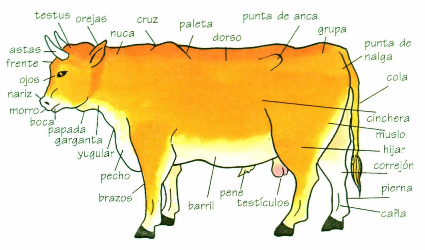
\includegraphics[scale=0.9]{img/dibujito1.png}
 \end{center}
 \caption{Partes físicas de un bovino. Tomada de \cite{librito1}}
\end{figure}

%%% Tek: faltan lsa refs para las figs

\subsubsection{Clasificación vacuna por aptitud productiva}
\begin{itemize}
\item \textbf{Lechero:} (Cabe resaltar que un requerimiento o propiedad fisonómica básica es que posean ubre, esto quiere decir solo las hembras pueden hacer parte de esta aptitud productiva). Poseen formación triangular, cuentan con cuerpo y extremidades largas y delgadas con poca voluminosidad cárnica
\begin{figure}[H]
 \begin{center}
 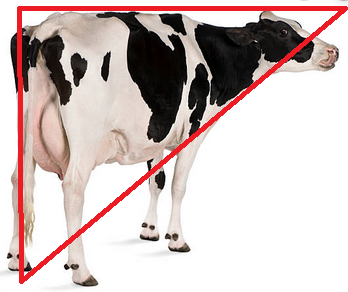
\includegraphics[scale=0.75]{img/dibujito2.png}
 \end{center}
 \caption{Aptitud lechera. Tomada de \cite{googlepics}. }
\end{figure}
\item \textbf{Carne:} Poseen una contextura rectangular. Además de poseer un cuerpo ancho con sus extremidades bien dotadas de carne.
\begin{figure}[H]
 \begin{center}
 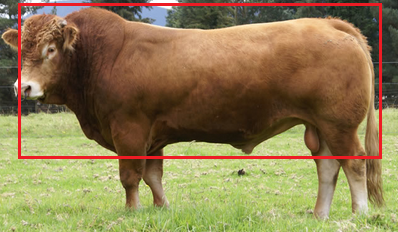
\includegraphics[scale=0.75]{img/dibujito3.png}
 \end{center}
 \caption{Aptitud de tipo carne. Tomada de \cite{googlepics}. }
\end{figure}
\item \textbf{Doble propósito:} Cuentan con propiedades mixtas de los 2 tipos ya mencionados, por lo que tanto su contextura, como volumen cárnico, ubre y extremidades son medianas. Este tipo de animales poseen una mayor facilidad en la adaptación del clima, alimentación y manejo. 
\begin{figure}[H]
 \begin{center}
 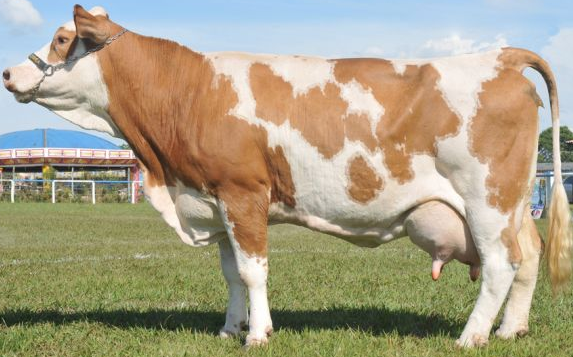
\includegraphics[scale=0.55]{img/dibujito4.png}
 \end{center}
 \caption{Aptitud de doble propósito.  Tomada de \cite{googlepics}. \label{}}
\end{figure}
\end{itemize}

% A modo general y para el desarrollo de este trabajo desde este punto en adelante, se decide describir más a fondo el ganado vacuno y enfocarse en describir de manera más profunda las ganaderías de la carne y la leche.\\


En el Cauca, aunque se cuente con abundantes hectáreas de diferentes fertilidades y condiciones térmicas apropiadas para el cultivo y desarrollo de la ganadería, se presentan muchas falencias en materia tecnológica y económica, en donde los movimientos migratorios de campesinos desplazados y los efectos colaterales del conflicto armado que se ha presentado en el país, son las principales causas de estas falencias. Sin embargo, el emprendimiento de los pequeños y medianos productores da paso a nuevas oportunidades de intervención por parte de la ingeniería y la implementación de nuevas metodologías que permitan mejorar la competitividad a la población campesina.\\

Lo anterior se diseña y se plantea acorde con el manual de Buenas Prácticas de Ganadería  (BPG) y con las legislaciones pertinentes al manejo de alimentos para el consumo humano establecidas por la ley colombiana mencionados en la Sección \ref{leyes}.

%%%%%%%%%%%%%%%%%%

\subsection{Sistemas de explotación del ganado vacuno}

Indiferentemente de su aptitud productiva, el ganado vacuno debe situarse en una infraestructura o ambiente apropiado para su desarrollo. Sin embargo, por  cuestiones geográficas, geológicas y/o climatológicas, los animales son criados mediante métodos de explotación como el estabulado, semiestabulado y el silvopastoril:

\begin{figure}[H]
 \begin{center}
 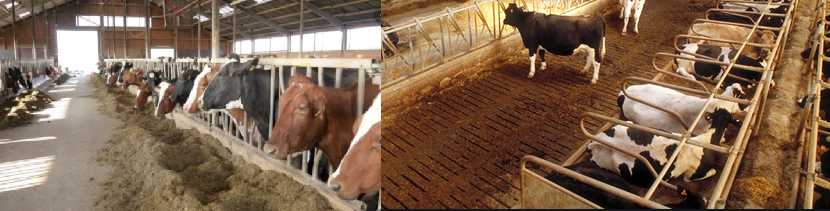
\includegraphics[scale=0.8]{img/estabulado.png}
 \end{center}
 \caption{Sistema de explotación estabulada. Tomada de \cite{googlepics}. \label{estabulpng}}
\end{figure}

El sistema ``estabulado'' (Ver Figura \ref{estabulpng}) es una forma de crianza de ganado en la cual los animales pasan la mayor parte del tiempo en establos donde realizan sus actividades diarias. En estos establos se recrea la vida del ganado con la diferencia que el mismo se encuentra protegido bajo techo sin tener exposición directa al sol y a las condiciones medio ambientales. En este sistema se pretende una mayor producción y mejor calidad de la carne en el menor tiempo posible \cite{defestabulacion}. Por su parte el sistema ``silvopastoril' (ver Figura \ref{silvopng})' es una forma de cultivo agropecuario que involucra la presencia de árboles interactuando con gramíneas y los animales sometidos a un manejo determinado para incrementar la productividad y el beneficio neto de la explotación a mediano y corto plazo \cite{defsilvopas}.

\begin{figure}[H]
 \begin{center}
 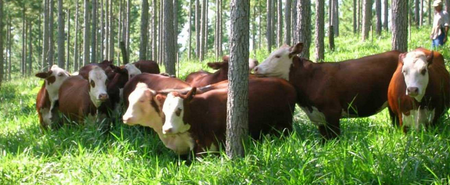
\includegraphics[scale=0.74]{img/silvopastoril.png}
 \end{center}
 \caption{Sistema de explotación silvopastoril. Tomada de \cite{contextoganadero}. \label{silvopng}}
\end{figure}

Finalmente, en el sistema semiestabulado se combinan los 2 sistemas mencionados. En este sistema mixto, los animales ingieren sus raciones de alimento principal en áreas extensas de pastos y forrajes vegetales, mientras que el cuidado y el suministro especializado de vitaminas y proteínas se realiza bajo techo.
%\begin{figure}[H]
% \begin{center}
% \includegraphics[scale=0.6]{img/tiposdosif.png}
% \end{center}
% \caption{Sistema de explotación por estabulación.  \label{estabulpng}}
%\end{figure}
%\begin{figure}[H]
% \begin{center}
% \includegraphics[scale=0.6]{img/tiposdosif.png}
% \end{center}
% \caption{Sistema de explotación silvopastoril. \label{silvopng}}
%\end{figure}
\subsection{Ciclo productivo de la leche}

% 2/10/2022 Cambiar la iamgen por una que tenga que ver con leche y luego descomentar el begin figure 
% \begin{figure}[H]
% \begin{center}
% 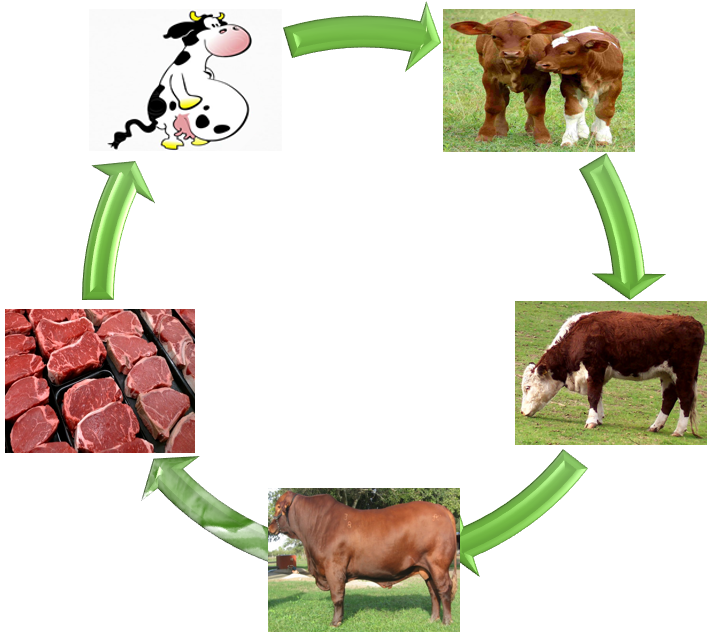
\includegraphics[scale=0.45]{img/ganadcarne.png}
% \end{center}
% \caption{Ciclo productivo en la ganadería de ordeño. \label{ganadcarnepng}}
% \end{figure}

% (Ver Figura \ref{ganadcarnepng}) 
 
El ciclo productivo de la leche de un ganado destinado para tal fin consta de 3 etapas principales que abarcan desde la gestación de la cría y maxima producción de leche, seguido de un periodo de declive y persistencia de producción y finalizando con el periodo de secado en donde se da descanso a la vaca para que se regenere el tejido glandular productor de leche para la siguiente lactancia \cite{mahecha}.\\

Estas etapas son brevemente descritas a continuación:


\begin{itemize}
    % \subsubsection{Etapa de crianza (Entre 0 y 2 años):} Es la 
    \item \textbf0{Etapa de crianza (Entre 0 y 2 años):} Es la etapa de producción temprana en donde el animal (generalmente crías hembras denominadas terneras) son alimentadas y criadas hasta alcanzar 2 años de edad.
	\begin{itemize}
% 		\item En esta etapa se requiere de grandes extensiones de tierra para producir crías
		\item No requiere de estaciones climatológicas específicas y se puede dar en todo el año (Esta característica varía dependiendo de la ubicación geográfica y las exposiciones climatológicas).
		\item Los elementos principales en la dieta de estas criaturas son los nutrientes provenientes del Calostro, la leche materna, forraje y vitaminas.\\
	\end{itemize} 
	% \subsubsection{Etapa de gestación y ordeño (Desde los 2 años en adelante y tras el primer parto respectivamente):} 
    \item \textbf{Etapa de gestación y ordeño (Desde los 2 años en adelante y tras el primer parto respectivamente):} Es la etapa inmediatamente siguiente a la etapa de crianza, en donde la novilla esta desarrollada y en la capacidad de ser inseminada para iniciar su producción de leche.
	\begin{itemize}
% 		\item En esta etapa se estima que el peso del animal puede alcanzar un mínimo de 230[kg] de peso en adelante.
% 		\item Es considerada como la etapa más rentable debido a las  pocas exigencias en materia de calidad alimenticia. 
		\item El objetivo de esta etapa es que la novilla produzca leche mientras que se da la gestación del novillo dentro de ella.
		\item El alimento se basa en pasturas de calidad, provenientes de las extensiones de tierra donde comen las reses y se crían.
		\item El animal gana mayor peso debido a su etapa de crecimiento, por lo que entre mejor sea su alimentación se obtendrán mejores resultados.
		\item Es de vital importancia que el animal se encuentre en la capacidad de  alimentarse \textit{Ad-Libitum}, es decir a placer y a voluntad.
		\item En caso de estar gestando su primera cría, la novilla es denominada ``primípara'', pues se encuentra abarcando el tiempo de gestación de su primera cría.\\
	\end{itemize} 
	% \subsubsection{Etapa seca o de secado:} Es la etapa final 
    \item \textbf{Etapa seca o de secado:} Es la etapa final que abarca los últimos 2 meses de gestación previos al parto en donde se da paso a la regeneración de tejidos glandulares que producen leche y a la curación de las glándulas mamarías para reducir el riesgo de mastitis. En sus características principales se pueden mencionar que aún cuando la novilla primípara esta en capacidad de producir leche, no se debe recurrir al ordeño hasta que no se realice el parto.
\end{itemize} 

\subsubsection{Razas}

Debido a la gran variedad de especies, condiciones ambientales, y al proceso evolutivo del ganado, históricamente se ha podido clasificar y seleccionar las razas más representativas para este tipo de explotación ganadera. Más precisamente se puede hacer mención de las siguientes:
\begin{multicols}{2}
    \begin{center}
        \begin{itemize}
        \item Simmental
        \item Holstein
        \item Jersey
        \item Normando
        \end{itemize}
    \end{center}
\end{multicols}

Éstas son seleccionadas principalmente por la contextura voluminosa pero factores como la calidad de la leche pueden sobrepasar los criterios cuantitativos. A continuación se muestran algunos ejemplares de estas razas:

\begin{figure}[H]
 \begin{center}
 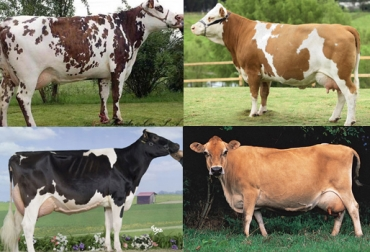
\includegraphics[scale=0.9]{img/razaslecheras.png}
% \end{center}
 \caption{En la primer fila de izquierda a derecha se observan ejemplares de las razas Normando, Simmental; seguido de las razas Holstein y Jersey en la fila inferior. Tomada de \cite{contextoganadero} \label{cuadrorazaspng}}
  \end{center}
\end{figure}

\subsection{Ciclo productivo de la carne}

\begin{figure}[H]
\begin{center}
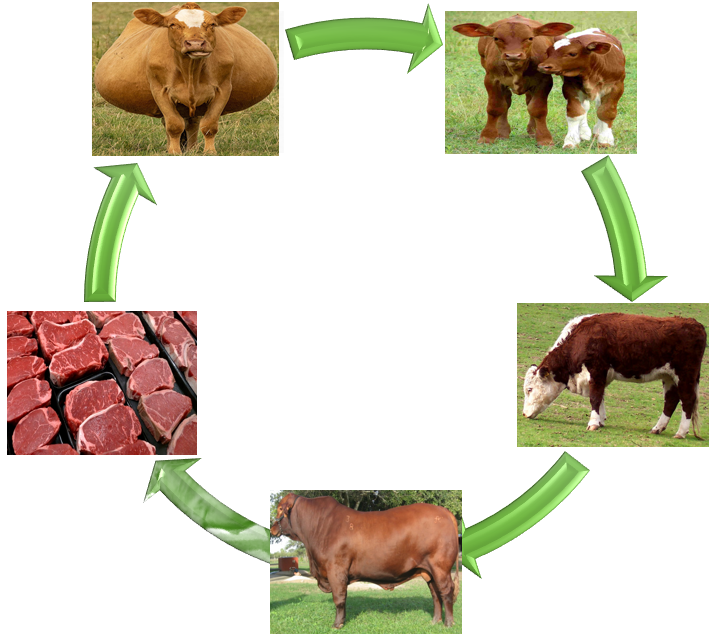
\includegraphics[scale=0.5]{img/ganadcarne2.png}
\end{center}
\caption{Ciclo productivo en la ganadería de la carne.  Modificada de \cite{contextoganadero}. \label{ganadcarnepng}}
\end{figure}

 
El ciclo productivo de la carne (Ver Figura \ref{ganadcarnepng})  de un ganado destinado para tal fin consta de 3 etapas principales que abarcan desde el nacimiento de la cría, su desarrollo y crecimiento y finalizando con su comercialización en el momento en que alcanza las condiciones apropiadas para ser transformado en carne para consumo humano \cite{mahecha}. Estas etapas son brevemente descritas a continuación:


%y finalizando en el momento en que alacanza las condiciones apropiadas para ser transformado en carne para consumo humano \cite{mahecha}. Estas etapas son brevemente descritas a continuación:

\begin{itemize}
	\item \textbf{Ganadería de Cría:} Es la etapa de producción temprana en donde el animal (generalmente crías macho llamadas bovinos) es alimentado y criado desde su nacimiento hasta los primeros seis (6) meses de edad. 
	\begin{itemize}
		\item En esta etapa se requiere de grandes extensiones de tierra para producir crías
		\item No requiere de estaciones climatológicas específicas y se puede dar en todo el año.
		\item Los elementos principales en la dieta de estas criaturas son los nutrientes provenientes del Calostro y la leche materna.\\
	\end{itemize} 
	\item \textbf{Ganadería de Levante:} Es la etapa inmediatamente siguiente a la etapa de crianza, en donde el bovino se desarrollará entre los siete (7) y diez y ocho (18) meses de edad.
	\begin{itemize}
		\item En esta etapa se estima que el peso del animal puede alcanzar un mínimo de 230[kg] de peso en adelante.
		\item Es considerada como la etapa más rentable debido a las  pocas exigencias en materia de calidad alimenticia. 
		\item El objetivo de esta etapa es que el sujeto en cuestión alcance el peso deseado en el menor tiempo posible con el menor esfuerzo posible
		\item El alimento se basa en pasturas de calidad, provenientes de las extensiones de tierra donde comen las reses y se crían.
		\item El animal gana mayor peso debido a su etapa de crecimiento, por lo que entre mejor sea su alimentación se obtendrán mejores resultados.
		\item Es de vital importancia que el animal se encuentre en la capacidad de  alimentarse \texit{Ad Libitum}, es decir a placer y a voluntad.\\
	\end{itemize} 
	\item \textbf{Ganadería de engorde o Ceba:} Es la etapa final que abarca desde los 19 meses de edad hasta los 24 o 36 meses, dependiendo de su crecimiento  y otros factores como el interés del productor, la demanda del mercado, entre otras. En sus características principales se pueden mencionar:
	\begin{itemize}
		\item El límite se define por los intereses del productor, la demanda del mercado y en general por el peso ideal del animal que es aproximadamente mayor o igual a los 450[kg].
		\item Para la alimentación se requieren de buenas, grandes y controladas cantidades con el fin de mejorar la carne. Para esto se utilizan dietas que requieren pasturas y concentrados dietarios.
		\item Se debe monitorear la alimentación tomando registro en la ganancia de gramaje diaria de cada uno de los animales.
	\end{itemize}
\end{itemize} 

\subsubsection{Razas} Debido a la gran variedad de especies, condiciones ambientales, y al proceso evolutivo del ganado, históricamente se ha podido clasificar y seleccionar las razas más representativas para este tipo de explotación ganadera. Más precisamente se puede hacer mención de las siguientes:
\begin{multicols}{4}
\begin{center}
\begin{itemize}
\item Beefmaster
\item Charolais
\item Simmental
\item Angus
\item Brangus
% \item Santa Gertrudis
\item Hereford
\item Limousin
\item Cebú
% \item Belgina Blue
\end{itemize}
\end{center}
\end{multicols}

Éstas son seleccionadas principalmente por la contextura voluminosa pero factores como la calidad de la carne pueden sobrepasar los criterios cuantitativos. A continuación se muestran algunas de las razas más usadas para este propósito:

\begin{figure}[H]
 \begin{center}
 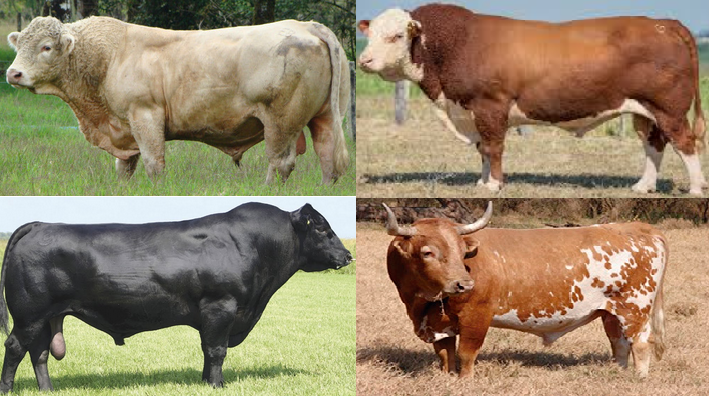
\includegraphics[scale=0.56]{img/cuadrorazas.png}
% \end{center}
 \caption{En la primer fila de izquierda a derecha se observan ejemplares de las razas Charolais, Hereford; seguido de las razas Angus y Criolla en la fila inferior.  Tomada de \cite{contextoganadero}. \label{cuadrorazaspng}}
  \end{center}
\end{figure}


\subsection{Alimentación y Componentes básicos de la dieta}
%\section{Marco de referencia}
% \subsubsection{Alimentación}
La alimentación de un cultivo de ganado requiere de una dieta o ración con diferentes componentes básicos o nutrientes que deben ser suministrados día a día de forma balanceada para lograr un crecimiento óptimo y que los animales puedan expresar su potencial genético \cite{recomendaciones}.\\

Los componentes principales que conforman la dieta alimenticia  del ganado son:
% 	\begin{itemize}
	

\subsubsection{Agua}
    Componente principal de la alimentación. Esta debe ser suministrada en cantidad y calidad para ser aprovechada por cada animal llegando a ocupar más del 50\% de la masa corporal de un ejemplar adulto y hasta un 90 \% de un recién nacido.
    	
	\begin{figure}[H]
	 \begin{center}
	 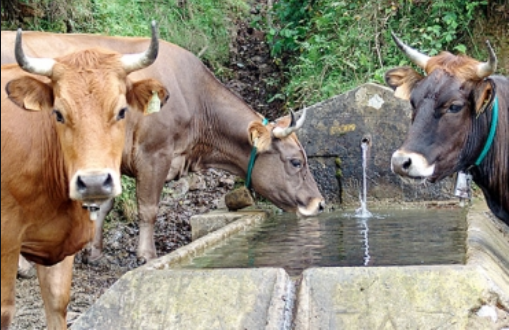
\includegraphics[scale=0.67]{img/agua.png}
	 \end{center}
	 \caption{Hidratación del ganado. Tomada de \cite{contextoganadero}.	\label{energeticospng}}
	\end{figure}
    	
\subsubsection{Energía}
Este componente se suministra mediante azúcares, almidones, celulosa, entre otros, los cuales aportan grandes cantidades de energía mas no de proteína, razón por la cual se deben suministrar de forma complementaria.
	\begin{figure}[H]
	 \begin{center}
	 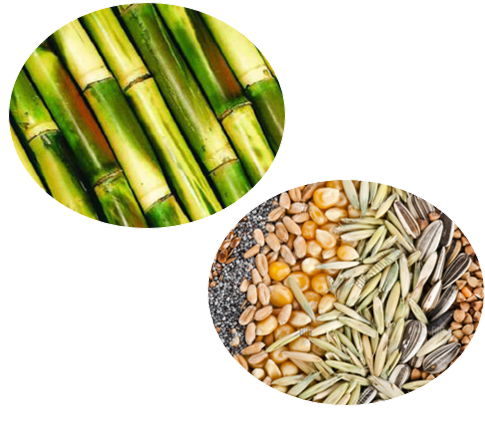
\includegraphics[scale=0.5]{img/melazacana.png}
	 \end{center}
	 \caption{Suplementos energéticos. 	\label{energeticospng}}
	\end{figure}
    
\subsubsection{Proteínas}
Estos nutrientes son fundamentales especialmente durante los periodos de sequía, por consiguiente, se optan por fuentes altas en proteína como leguminosas forrajeras, el Maní, Leucaena y el más común, los pastos de forraje verde. 
	\begin{figure}[H]
	 \begin{center}
	 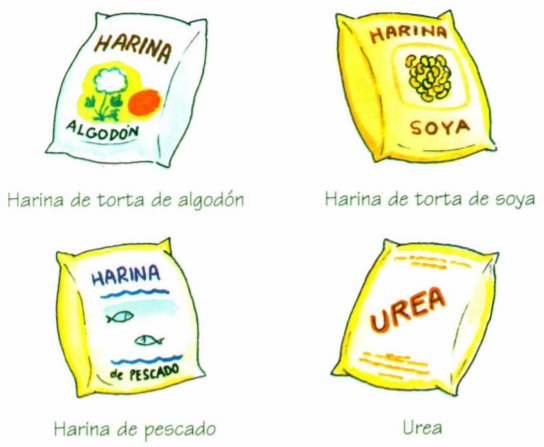
\includegraphics[scale=0.8]{img/proteina.png}
	 \end{center}
	 \caption{Suplementos proteínicos. Tomada de \cite{librito1}. \label{proteinaspng}}
	\end{figure}

\subsubsection{Minerales}
Son indispensables en la ganancia de peso de los novillos durante la etapa de Cría y Levante. Este complemento alimenticio debe estar siempre a la disposición para que el ganado pueda abastecer sus necesidades. Estos minerales se suelen proporcionar mediante mezclas de macrominerales y microminerales que se ofrecen de libre consumo al ganado.

\subsubsection{Vitaminas}
Suministradas en cantidades pequeñas aplicadas comúnmente en animales cuya alimentación se basa en forrajes secos,  o en animales enfermos convalecientes, desnutridos o durante épocas de sequía prolongada.
	\begin{figure}[H]
	 \begin{center}
	 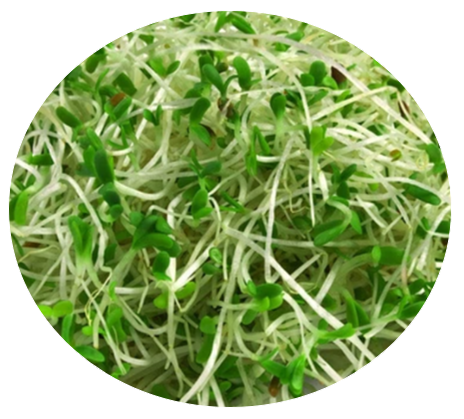
\includegraphics[scale=0.6]{img/leguminosas.png}
	 \end{center}
	 \caption{Forraje y leguminosas. Tomada de \cite{librito1}. \label{vitaminaspng}}
	\end{figure}

\subsection{Balance de raciones y dietas especializadas}
% \subsubsection{Balance de raciones y dietas especializadas}
    Estas dietas son suministradas por personal técnico calificado que prepara un dieta acorde a la cantidad de nutrientes de cada animal de forma particular e independiente, considerando su peso actual, su velocidad de crecimiento y estado fisiológico.

% \subsection{Desperdicios} Hablar de desperdicios ?

\subsection{Leyes y Normatividad}  \label{leyes}
Requerida para que el avance ganadero se realice de manera coordinada o estandarizada basada en las buenas prácticas ganaderas (Decreto 072 de 2007) en pro de mejorar la productividad y ayudarla a alcanzar niveles de ganadería bovina del mundo \cite{invima}, \cite{leylacteos}, \cite{minsaludleche}. 
\begin{itemize}
	% \item \textbf{Resolución 2310 de 1986:} Reglamentación parcial en el título V de la ley 09 de 1979 que se refiere al procesamiento, composición, requisitos, transporte, y comercialización de los Derivados Lácteos.
	% \item \textbf{Resolución 11961 de 1989:} Reglamentación parcial a la resolución 2310 de 1986 que se refiere a lo relacionado con las clases de leche fermentada.
	% \item \textbf{Decreto 0616 de 2006:} Reglamento técnico sobre los requisitos que debe cumplir la leche para el consumo humano que se obtenga, procese, envase, transporte, comercialice, expenda, importe o exporte en el país.
	\item \textbf{Resolución 0012 de 2007:} Por la cual se establece el sistema de pago de la leche cruda al productor, diseñado por la Unidad de Seguimiento de Precios.
	% \item \textbf{Decreto 1500 de 2007:} Reglamento técnico a través del cual se crea el Sistema Oficial de Inspección, Vigilancia y Control de la Carne y otros productos comestibles y derivados cárnicos destinados para el consumo humano.
	% \item \textbf{Decreto 072 de 2007:} Por el cual se establece el manual de buenas prácticas de manejo para la producción de ganado bovino.
	% \item \textbf{Decreto 2905 de 2007:} Por el cual se establece el reglamento técnico sobre los requisitos sanitarios y de inocuidad de la carne y productos cárnicos comestibles de las especies bovina y bufalina destinados para el consumo humano.
	% \item \textbf{Decreto 18119 de 2007:} Por el cual se reglamenta los requisitos del plan gradual de cumplimiento para  las plantas de beneficio y desposte de bovino y bufalinos.
	% \item \textbf{Decreto 2278 de 1982:} Reglamentación parcial en el titulo V de la ley 09 de 1979 que se refiere al sacrificio de animales de abasto público o para consumo humano y el procesamiento, transporte y comercialización de su carne.

\end{itemize}

\section{Modelación matemática} \label{modmatsec}
% \textbf{PONER TODA LA INFO TEÓRICA DE CADA TEMA, }
\subsection{Regresión lineal}
La regresión lineal es un método estadístico usado para modelar la relación entre una variable dependiente denotada como $y$ y una o más variable dependientes dentadas como $x_{i}$. El objetivo de este método es encontrar una ecuación lineal que mejor represente cómo las variables independientes influencian a la variable dependiente. La ecuación lineal estimada se puede definir como en la Ecuación \#\ref{eqreglin}:

\begin{equation*}
    y = \beta_{0} + \beta_{1}x_{1} + \beta_{2}x_{2} + \beta_{3}x_{3} + ... + \beta_{n}x_{n} + \epsilon
\end{equation*}
\begin{equation}
    y = \beta_{0} + \sum_{i=1}^{n}(\beta_{i}x_{i}) + \epsilon \label{eqreglin}
\end{equation}

Donde $y$ es la variable independiente, $x_{i}$ son las variables independientes, $\beta_{i}$ son los coeficientes a estimar; y $\epsilon$ representa el término de error por posibles variaciones en la variable dependiente $y$. El objetivo de este método es encontrar los valores de los coeficientes $\beta_{i}$ que minimizan la suma de las diferencias cuadradas entre los valores observados de la variable dependiente $y$ y los valores predichos por la ecuación. Típicamente se logra utilizando el método de regresión por mínimos cuadrados.

\subsection{Regresión no lineal}

En comparación al método de regresión lineal, cuando la variable dependiente posee una naturaleza no lineal, el método estadístico usado para encontrar las relaciones entre las variables independientes $x_{i}$ y la variable dependiente $y$ es denominado como regresión no lineal. En este tipo de regresión se utiliza una función $f(x_{i};\theta)$ con variables independientes $x_{i}$ y parámetros $\theta$, que puede tener distintas formas dependiendo del problema. Una forma general de describir un modelo de regresión no lineal es:

\begin{equation}
    y = f(x_{i};\theta) + \epsilon
\end{equation}

Donde $y$ es la variable independiente, $x_{i}$ son las variables independientes, $\theta_{i}$ son los parámetros a estimar; y $\epsilon$ representa el término de error por posibles variaciones en la variable dependiente $y$. En este caso el objetivo de este método es encontrar los valores de los parámetros $\theta$ y del error $\epsilon$ de tal forma que los valores estimados de $y$ se ajusten a los datos existentes. Aún cuando la regresión lineal es directa e intuitiva, este tipo de aproximación solo es valida cuando la incertidumbre no esta relacionada ni con la variable independiente ni con la variable dependiente por lo que no es muy útil para situaciones en las que los datos han sufrido transformaciones \cite{nlreg}. Para ello pueden utilizarse otros tipos de regresión tales como la polinómica, Splines cúbica, entre otras (ver ejemplo comparativo en la Figura \ref{splinesfig}).

\subsection{Interpolación con Splines}
Los splines son un enfoque matemático y computacional usado en el ajuste e interpolación de curvas tanto lineales como no lineales. Dado su naturaleza, las splines son funciones matemáticas que describen el dominio de una curva dividiéndola en segmentos representados por funciones polinómicas por partes de bajo orden. Cuando éstas funciones son de bajo orden, son usadas para representar de manera sencilla a funciones lineales, y cuando son de alto orden (por lo general cúbicas), son usadas para representar de manera precisa a las curvas de funciones no lineales.

\subsubsection{Splines cúbicas}\label{splinescub}

Los splines cúbicos son splines en los que cada segmento está representado por una función polinómica cúbica, siendo este el grado máximo del polinomio en cada tramo. Suponiéndose un conjunto de puntos de datos ($x_{i}$, $y_{i}$), se utilizan splines cúbicos para construir un polinomio cúbico por partes que pasa por cada dupla de valores, además de existir primera y segunda derivada continua en cada pareja de datos, de esta forma se asegura una curvatura suave y visualmente atractiva (ver Figura \ref{splinesfig}). La definición matemática de cada segmentos entre cada par de valores ($x_{i}$,$x_{i+1}$) se representa de la siguiente manera:

\begin{equation}
    S_{i}(x)=a_{i} + b_{i}(x-x_{i}) + c_{i}(x-x_{i})^{2} + d_{i}(x-x_{i})^{3}
\end{equation}

Donde $S_{i}(x)$ es la función de spline cúbica para el segmento $i-$ésimo, $a_{i}$, $b_{i}$, $c_{i}$ y $d_{i}$ son los coeficientes específicos para el segmento $i-$ésimo. 

\begin{figure}[h]
    \centering
    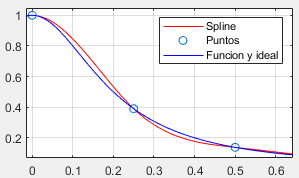
\includegraphics[scale=1.18]{img/splines.png}
    \caption{Comparación entre una interpolación de datos por Splines Cúbicas vs Una función polinómica ideal}
    \label{splinesfig}
\end{figure}


\pagebreak

\subsection{Ajuste de curvas}

El ajuste de curvas es un proceso matemático y estadístico que determina la curva o función de mejor ajuste que describe a un conjunto puntos. El objetivo principal de esta técnica consiste en encontrar el modelo matemático que se aproxime a la relación existente en los datos entre la variable independiente y la variable dependiente. De esta forma puede que se establezcan valores de la variable dependiente que pueden no estar presentes en el conjunto de datos original. El ajuste de curvas también involucra la estimación de valores inexistentes o ausentes entre los puntos de datos haciendo uso de técnicas de interpolación. El modelo matemático utilizado esta determinado por la naturaleza de los da tos y el problema que se desea satisfacer, y este ajuste puede ser logrado tanto por modelos lineales así como también modelos no lineales que dependerán de la naturaleza de la conexión entre la variable independiente, comúnmente $x$ y la variable dependiente, comúnmente $y$.

\subsection{Métodos de ajuste no lineal}
En los casos en los que un modelo linea no es puede capturar efectivamente la conexión entre las variables, se aplican métodos de ajuste de curvas no lineales. Estos métodos implican ajustar funciones no lineales a los datos para capturar relaciones más complejas \cite{curvefitdalgaard}. Entre los métodos más comunes de ajuste de curvas no lineales podemos encontrar al ajuste por mínimos cuadrados no lineales (en inglés, Nonlinear Least Squares ó NLS), en donde éste método minimiza la suma de las diferencias cuadradas entre los valores observados y los valores estimados, el ajuste de suavizado de curvas exponenciales, usualmente utilizado cuando los datos evidencian un crecimiento o decrecimiento exponencial, el ajuste de curvas logísticas, frecuentemente usados en casos donde se presentan modelos de crecimiento y/o fenómenos de saturación con curvas de comportamiento sigmoideo, el método de Gauss-Newton, comúnmente usado en ingeniería para lograr la regresión no lineal mediante una optimización iterativa; entre otros métodos explicados a continuación.


\subsubsection{Algoritmo de ``Levenberg-Marquardt'' (LMA)}\label{LMAlabel}

El algoritmo de Levenberg-Marquardt (LMA), comúnmente conocido como el enfoque de mínimos cuadrados amortiguados, en inglés: ``Damped Least Squares'' (DLS, por sus siglas en inglés), es una metodología matemática y computacional utilizada para manejar problemas de mínimos cuadrados no lineales, especialmente el ajuste de curvas. Cuando intentamos identificar los parámetros de mejor ajuste para una curva modelo dada que minimiza la suma de los cuadrados de las desviaciones entre los puntos de datos observados y la curva, nos encontramos con varias dificultades de minimización. Si un modelo es lineal en sus parámetros, el objetivo de mínimos cuadrados es cuadrático en los parámetros.\\

Este objetivo puede minimizarse con respecto a los parámetros en un solo paso mediante la solución de una ecuación matricial lineal. Este tipo de solución reduce la suma de los cuadrados de los errores entre la función del modelo y los puntos de datos a través de una secuencia de actualizaciones bien elegidas de los valores de los parámetros del modelo \cite{levenberduke}. Siguiendo el método de Gauss-Newton (GNA), la suma de los errores al cuadrado se reduce asumiendo que la función de mínimos cuadrados es localmente cuadrática en los parámetros y encontrando el mínimo de esta cuadrática. Esta medida de bondad de ajuste con valores escalares se denomina criterio de error de chi-cuadrado ($\chi^{2}$), porque la suma de los cuadrados de las variables aleatorias normalmente distribuidas se distribuye como la distribución de ($\chi^{2}$). Si la función $y$ es no lineal en los parámetros del modelo, entonces la minimización con respecto a los parámetros debe realizarse de forma iterativa \cite{levenberduke}. \\

El ajuste de curvas es un proceso que se utiliza para encontrar una función matemática que mejor se ajuste a un conjunto de datos experimentales. Una de las técnicas más populares para el ajuste de curvas es el algortimo de Levenberg-Marquardt (LMA), que es una combinación de los métodos de GNA y el método del gradiente conjugado \cite{levenberduke}. El método de LMA es muy eficiente en la resolución de problemas de ajuste de curvas no lineales, y es ampliamente utilizado en diversas áreas de la ciencia incluyendo la física, la química, la biología, la economía y la ingeniería.\\


En términos generales, el método de LMA se basa en un enfoque iterativo que comienza con una estimación inicial de los parámetros de la función de ajuste y se ajusta sucesivamente hasta que se alcanza una solución que minimiza la función de error cuadrático, incluso si comienza lejos del mínimo final. Este método utiliza una matriz jacobiana para calcular la dirección del gradiente y la tasa de aprendizaje de cada paso iterativo. Si la tasa de aprendizaje es grande, el método funciona como el método del gradiente conjugado. Si la tasa de aprendizaje es pequeña, el método funciona como el método de Gauss-Newton. Por lo tanto, el método de Levenberg-Marquardt es una combinación de ambos métodos \cite{levenberduke}. Este problema puede formularse matemáticamente como:

\begin{align}
\text{Min} \quad & \sum_{i=1}^{N} [y_i - f(x_i; \theta)]^2,
\end{align}

Donde $y_i$ es la variable dependiente observada, y $f(x_i; \theta)$ representa la función del modelo con los parámetros $\theta$. El objetivo es minimizar la suma de los cuadrados de las desviaciones entre la variable dependiente observada $y_i$ y la función modelo $f(x_i; \theta)$ con parámetros $\theta$, tomados en todos los puntos de datos ($i = 1$ a $N$).

\subsubsection{Algoritmo de ``Efectos Mixtos No Lineales'' (NLMEA)}\label{NLMEAlabel}

Otro de los métodos de ajuste más utilizados para el análisis individualizado de múltiples objetivos dependientes del tiempo es el ajuste por efectos mixtos lineales y no lineales. Estos modelos de efectos mixtos se basan en un modelo generalizado para describir poblaciones aún cuando los parámetros de crecimiento del modelo pueden ser únicos para los sujetos de estudio \cite{mixedShelley}. El modelado con el Algoritmo de Efectos Mixtos No Lineales (Nonlinear Mixed Effects Algorithm ó NLMEA, por sus siglas en inglés) es una técnica estadística para analizar datos que presentan mediciones repetidas o patrones jerárquicos. Es especialmente útil cuando se trata con datos que contienen varianzas individuales y heterogeneidad. El método NLMEA amplía los modelos clásicos de regresión no lineal al incluir efectos fijos (Nonlinear Mixed Effects Algorithm - Fixed Effects ó NLMEA-FE, por sus siglas en inglés) donde se identifican parámetros a nivel de población; así como efectos aleatorios (Nonlinear Mixed Effects Algorithm - Random Effects ó NLMEA-RE, por sus siglas en inglés ) donde se identifican parámetros específicos asociados a cada sujeto estudiado, lo que permite tener en cuenta tanto la variabilidad entre individuos como la variabilidad dentro de cada individuo en el tiempo. Para este método, agregar efectos aleatorios a un modelo extiende la confiabilidad de las inferencias más allá de la muestra específica de individuos.\\

Considerando un modelo no lineal con parámetros específicos para cada individuo, el modelo NLMEA se representa matemáticamente de la siguiente manera:

\begin{equation}
y_{ij} = f(x_{ij}; \theta_i) + \varepsilon_{ij}    
\end{equation}

Donde $y_{ij}$ es la respuesta observada para la medición  $j-$esima en el individuo $i-$esimo. $x_{ij}$ Es la correspondiente variable predictora para la medición $j-$esima en el individuo $i-$esimo. $f(x_{ij}$, $\theta_{i})$ representa el modelo no lineal con parámetros específicos para cada individuo ($\theta_{i}$). $\varepsilon_{ij} $ es el termino de error aleatorio que se asume con distribución normal con media cero (0) y varianza constante.\\

% Los modelos de efectos mixtos tienen en cuenta tanto los efectos fijos como los aleatorios. Así como todos los modelos de regresión, su propósito es describir una variable de respuesta en función de las variables predictoras; sin embargo, los modelos de efectos mixtos reconocen las correlaciones dentro de los subgrupos de muestra. %(no aplicable para este caso pues no los sujetos de estudio son las reses individuales y no hay subgrupos).
% De esta manera, proporcionan un compromiso entre ignorar los grupos de datos por completo y ajustar cada grupo con un modelo separado \cite{matlabmixed}.

El modelado por NLMEA intenta estimar tanto los parámetros a nivel de población como los parámetros específicos de cada individuo al mismo tiempo. El modelo incorpora la variabilidad poblacional al tener en cuenta influencias aleatorias, lo que permite calcular la variación individual aparte de reconocer las correlaciones dentro de los subgrupos de muestra. El enfoque NLMEA se utiliza con frecuencia en una variedad de campos, incluyendo la farmacocinética, la investigación longitudinal y el modelado de crecimiento, donde la variabilidad individual y las mediciones repetidas son propiedades comunes de los datos.

% \begin{itemize}
%     \item \textbf{``Efectos Mixtos Fijos'' (EM-F):}
%     \item \textbf{``Efectos Mixtos Aleatorios'' (EM-A):}
% \end{itemize}

\subsection{Modelación por ``Ecuaciones Diferenciales Ordinarias'' (EDOs)}\label{EDOlabel}
Este es un enfoque matemático utilizado para representar, analizar y evaluar sistemas dinámicos en los que el comportamiento de un sistema está influenciado por su estado actual, su evolución en el tiempo, los factores de entrada involucrados y las respuestas a estos estímulos. Las EDOs son ampliamente usadas en múltiples disciplinas científicas tales como la ingeniería, la física, la biología, entre otras. Las EDOs permiten modelar los cambios presentes en un sistema en donde se presentan tasas de cambio de una o más variables dependientes con respecto a sus valores existentes.\\

Dependiendo del orden del modelo, las EDOs pueden clasificarse en primer orden al considerar la primer derivada de la variable, ó de orden superior cuando se involucran derivadas de orden 2 o superior \cite{mathmod1D}. \pagebreak


\subsubsection{Planteamiento de un modelo por EDOs}

Para proponer un modelo por ecuaciones diferenciales ordinarias es necesario tener en cuenta las siguientes consideraciones:
\begin{enumerate}
    \item \textbf{Definir el sistema:} Se deben definir el sistema que se desea modelar, las variables clave y las relaciones existentes entre éstas.
    \item \textbf{Formular las EDOs:} Se debe escribir las ecuaciones que describen los cambios o evoluciones que presentan las variables con respecto a otra variable, comúnmente dependientes del tiempo.
    \item \textbf{Específicar parámetros:} Se deben asignar valores o rangos para los parámetros incluidos en las EDOs, estos parámetros influenciarán significativamente al comportamiento del sistema.
    \item \textbf{Condiciones iniciales:} Estos son los valores iniciales de las variables dependientes en la primer muestra, comúnmente en tiempo $t=0$.
    \item \textbf{Viabilidad:} Dependiendo de la complejidad del modelo, es posible que pueda ser solucionado de manera determinista, o mediante el uso de métodos numéricos y simulaciones computacionales.
    \item \textbf{Validación y análisis:} Verificar si es posible validar el modelo frente a datos o resultados experimentales, analizando el comportamiento del modelo frente a diferentes condiciones.
    
\end{enumerate}
% \subsection{Modelamiento EDO: Balance de energía}

% % Para ejemplificar el planteamiento de un modelo  con EDOs se procede a determinar las ecuaciones que simulan el comportamiento de un péndulo de Furuta.
% % \subsubsection{Modelación por EDO de un péndulo de Furuta}

% % El péndulo de Furuta rotacional se compone de 2 brazos que realizan movimiento rotacionales en 2 planos perpendiculares. El primer brazo, el brazo del motor, realiza movimientos rotacionales entre los ejes \textbf{x} y \textbf{y}; mientras que el segundo brazo, el brazo del pendulo,  realiza movimientos rotacionales entre el eje \textbf{z} y el plano \textbf{xy}.\\

% % \begin{figure}[h]
% %     \centering
% %     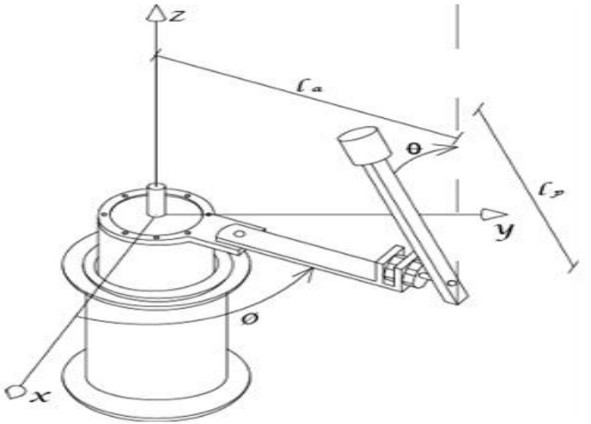
\includegraphics[scale = 0.7]{img/furutapen.jpg}
% %     \caption{Referenciación espacial del péndulo de Furuta.}\label{nonlin}
% % \end{figure}

% % En vista que la demostración matemática de este tipo de modelación por EDOs no es la cuestión principal de este trabajo de grado, ésta se anexa al final de este trabajo.\\

% % Mediante la ecuación de Euler-Lagrange, se puede establecer el balance de energías presentes en este modelo, siendo estas la energía cinética y la energía potencial, en donde las ecuaciones \ref{ecinetica} y \ref{epotencial} describen su comportamiento para este caso:

% % \begin{equation}
% %     E_{kb}=\frac{m_{bm}v_{bm}^{2}}{2} + J_{bm}\dot{\theta}^{2}, \hspace{0.25cm} E_{kp}=\frac{m_{p}v_{p}^{2}}{2} + \frac{I_{zz}w_{p}^{2}}{2},\hspace{0.25cm} I_{zz}=J_{p} \label{ecinetica}
% % \end{equation}
% % \begin{equation}
% %         E_{pp}=m_{p}gL_{p}\left(cos(\phi)-1\right) \label{epotencial}
% % \end{equation}

% % Donde $J_{p}$ y $J_{bm}$ son las inercias del péndulo y del brazo del motor, $w_{p}$ es la velocidad total del péndulo ($V_{totp}$). Esta velocidad total del péndulo es resultante  de la suma de la velocidad del ángulo del péndulo junto con la velocidad del ángulo del brazo del motor. $L_{p}$ es el largo del brazo del péndulo, $L_{b}$ es el largo del brazo unido al motor, $m_{bm}$ es la masa del brazo unido al motor, $m_{p}$ es la masa del brazo del péndulo, $\phi$ es la posición angular del brazo del motor y \dot{\phi} su velocidad; análogamente, $\theta$ es la posición angular del brazo del motor y \dot{\theta} su velocidad.
% % % Para este tipo de péndulos se busca medir las posiciones angulares de los brazos y sus respectivas velocidades (derivadas). Por lo tanto es imprescindible establecer un punto de referencia para modelar este sistema.

% % % Comenzando por expresar los ejes cartesianos del brazo del motor mediante coordenadas polares se obtiene que:

% % % \begin{equation*}
% % %         x = rcos\left(\phi\right), \hspace{0.25 cm} y = rsin\left(\phi\right), \hspace{0.25 cm} z = 0
% % % \end{equation*}

% % % Obsérvese que para el brazo del motor, denominado como r, no se tienen movimientos rotacionales en el eje Z por lo tanto $z = 0$.

% % % En cuanto al eje de referencia del péndulo los ejes de referencia se expresarían así: \textbf{(poner imagen del péndulo con vista frontal)}

% % % \begin{equation*}
% % %         x = rcos\left(\phi\right)-L_{p}sin\left(\phi\right)sin\left(\theta\right), \hspace{0.25 cm} y = rsin\left(\phi\right)+L_{p}sin\left(\theta\right)cos\left(\phi\right), \hspace{0.25 cm} z = L_{p}cos\left(\theta\right)% - L_{p}
% % % \end{equation*}

% % % Se debe tener en cuenta que el punto de origen para este eje de referencia es el extremo del brazo del motor.

% % Como lo sugiere \cite{mees}, una manera sencilla pero eficaz de establecer un modelo EDO para simular un sistema, es mediante el balance de energías que entran y salen del sistema. De esta forma se puede establecer que 


% \subsubsection{Ajuste de modelos EDO}

% \subsubsection{Optimización de modelos EDO}

\subsection{Criterios de evaluación}
\subsubsection{Error Cuadrático Medio (MSE) y Raíz de Error Cuadrático Medio (RMSE)}
El MSE y el RMSE son métricas típicamente utilizadas en estadística y en modelos de aprendizaje automático (``Machine learning'' en inglés) que sirven para evaluar la precisión del modelo estimador. Por su parte, el MSE mide la diferencia cuadrática promedio entre los valores observados (reales) y los valores esperados (teóricos). El MSE se calcula como el promedio del cuadrado de  los residuos tal y como se observa a continuación:

\begin{equation}
    MSE = \frac{1}{n} \sum_{i=1}^{n}(y_{i}-\hat{y_{i}})^{2}
\end{equation}

Este criterio es comúnmente usado en problemas de regresión para evaluar la bondad de ajuste del modelo. En pocas palabras, la interpretación de está métrica indica que entre menor sea el valor, mejor es el ajuste. No obstante, Es importante considerar que al elevar los errores al cuadrado, se penalizan los errores más grandes a comparación de los errores pequeños ocasionando que este criterio sea sensible a datos atípicos. Por su parte el RMSE se obtiene aplicando la raíz  cuadrada al MSE, este proceso se realiza teniendo en cuenta que mejora su interpreta ción puesto que las unidades de esta métrica son las mismas que las de los datos usados \cite{msereg}.

\subsubsection{Máxima verosimilitud ($\log \mathcal{L}$)}

La estimación por máxima verosimilitud es una medida que permite saber qué tan bien un modelo estadístico explica los datos observados. Este criterio cuantifica la probabilidad de observar los datos bajo los supuestos del modelo. Se cree que los modelos que poseen mayores probabilidades logarítmicas se ajustan mejor a los datos. En muchos escenarios, la estimación de parámetros estadísticos implica maximizar la probabilidad logarítmica, como resultado se obtienen estimaciones de máxima verosimilitud de los parámetros del modelo. Para calcular la máxima verosimilitud de un modelo se debe:
\begin{enumerate}
    \item Calcular la verosimilitud para un única observación $x_{i}$ obteniéndose:
    \begin{equation*}
        \mathcal{L}(x_{i}|\mu,\sigma) = \frac{1}{\sqrt{2\pi\sigma^{2}}} e^{-\frac{(x_{i}-\mu)^{2}}{2\sigma^{2}}}
    \end{equation*}
    \item Suponiéndose que hay independencia entre los datos, se calcula la verosimilitud de todo el conjunto de datos de la siguiente manera
    \begin{equation*}
        \mathcal{L}(x_{1},x_{2},...,x_{n}|\mu,\sigma) = \prod_{i}^{n}\mathcal{L}(x_{i}|\mu,\sigma)
    \end{equation*}
    \item Finalmente, se procede a determinar el logaritmo natural para obtener la verosimilitud logarítmica, obteniéndose que:
    \begin{equation}
        \log\mathcal{L}(x_{1},x_{2},...,x_{n}|\mu,\sigma) = \sum_{i}^{n}\left[-\left(\frac{1}{2}\right)\log(2\pi\sigma^{2})-\frac{(x_{i}-\mu)^{2}}{2\sigma^{2}}\right]
    \end{equation}
\end{enumerate}

\subsubsection{ Criterio de Información de Akaike (AIC)}\label{aiclabel}

El criterio de información de Akaike en un modelo estadístico es la medida para la calidad de ajuste del modelo. Este logra un balance entre ajuste y complejidad del modelo, esto quiere decir, un balance entre una buena captura de datos y el número de parámetros usados. El AIC mide qué tan bien se ajusta el modelo a los datos y al mismo tiempo penaliza la complejidad para evitar el sobreajuste (``overfitting'' en inglés). En esencia, el criterio AIC es utilizado para comparar y elegir modelos candidatos y dependiendo de su valor, se puede sugerir un mejor equilibrio entre el ajuste y la simplicidad del modelo \cite{aicbicdata}. Este criterio se puede calcular mediante la siguiente ecuación:

\begin{equation}
    AIC = -2\ln(\mathcal{L})+2k
\end{equation}
Donde $\mathcal{L}$ es la función de máxima verosimilitud, $k$ es la cantidad de parámetros, para un tamaño de muestra $n$.

\subsubsection{Criterio de Información Bayesiano (BIC)}\label{biclabel}

También conocido como el criterio de información de Schwarz, es un criterio similar al AIC pero éste criterio aplica una mayor penalización en la complejidad del modelo. El uso de este criterio esta enfocado en la selección de modelos, especialmente cuando se necesita  una penalización más estricta por la complejidad del modelo. A diferencia del AIC, el BIC favorece a los modelos más simples, lo que lo hace más eficaz al momento de seleccionar un modelo candidato \cite{aicbicdata}. Para calcular este criterio, se debe:

\begin{equation}
    BIC = -2\ln(\mathcal{L})+2k\ln(n)
\end{equation}
Donde $\mathcal{L}$ es la función de máxima verosimilitud, $k$ es la cantidad de parámetros, para un tamaño de muestra $n$.


\subsubsection{``Chi-cuadrado'' ($\chi^{2}$) y ``Chi-cuadrado'' reducido ($\chi^{2}_{red}$)}

\begin{itemize}
    \item \textbf{Factor $\chi^{2}$:} Este es un número real que \textbf{no puede ser negativo} y se determina sumando las diferencias al cuadrado entre los valores observados y predichos, dividiendo el resultado por los valores esperados (ver Ecuación \ref{formulachi}). El objetivo princiapl de la prueba de $\chi^{2}$ se utiliza para determinar si existe o no una diferencia estadísticamente significativa entre los valores observados y estimados. Un valor de $\chi^{2}$ bajo sugiere una estrecha coincidencia entre los valores observados y esperados, lo que indica un buen ajuste, en caso contrario el ajuste sería deficiente.
    \begin{equation}
        \chi^{2} = \sum_{i=1}^{n}\frac{\left(O_{i}-E_{i}\right)^{2}}{E_{i}} \label{formulachi}
    \end{equation}
    Donde $O_{i}$ representa el valor observado para un valor específico y $E_{i}$ representa el valor esperado para un valor en específico. Es importante considerar los grados de libertad (degrees of freedom en inglés ó DOF) que se definen como el número de categorías o valores menos 1, y esto es lo que determina la forma de la distribución $\chi^{2}$. Por En cuanto a la bondad de ajuste, $\chi^{2}$ es usado para evaluar qué tan bien los datos observados se ajustan a los valores estimados por el modelo teórico.
    \item \textbf{Factor $\chi^{2}$ reducido:} Este es una versión modificada del factor $\chi^{2}$ que hace referencia al número de grados de libertad en un test estadístico. Este valor es comúnmente usado para comparar modelos con distinta cantidad de parámetros con el objetivo de evitar el sobreajuste de los datos. Para calcular el factor $\chi^{2}$ reducido se debe dividir el factor $\chi^{2}$, por el número de grados de libertad:
    \begin{equation}
        \chi_{red}^{2} = \frac{\chi^{2}}{DOF}
    \end{equation}
    \textbf{El factor decisivo radica en escoger el modelo que cuente con el valor más pequeño de $\chi_{red}^{2}$} implicando que ese modelo brinda un mejor balance entre la bondad de ajuste y la simplicidad del modelo.
\end{itemize}

\section{Descripción general del proyecto realizado bajo la metodólogía CRISP-DM}

Tal y como se mencionó en la Sección \ref{crispmethod} La metodología CRISP-DM se compone de distintas etapas, comenzando desde el entendimiento del negocio  hasta completar el despliegue e implementación de los modelos obtenidos. Para tener una perspectiva general del desarrollo general de este proyecto se plantea un diagrama de bloques general evidenciado en la Figura \ref{tesispptsenapng}. En éste diagrama se quiere mostrar cómo se ha planteado el desarrollo de las etapas de Entendimiento de los datos, Preparación de datos, Modelación y Evaluación, las cuales componen la estructura principal del desarrollo de este proyecto. La primer etapa no son consideradas dentro de este diagrama en tanto que la etapa inicial de Entendimiento del negocio, la cual se logra bajo el entendimiento del contexto al rededor del negocio, no están bajo el control del autor; esto mismo sucede para la etapa de despliegue, pues esta decisión depende únicamente del SENA quien tomará la decisión de implementar (o no) las ventajas que ofrece este proyecto de investigación. 

\begin{figure}[H]
    \centering
    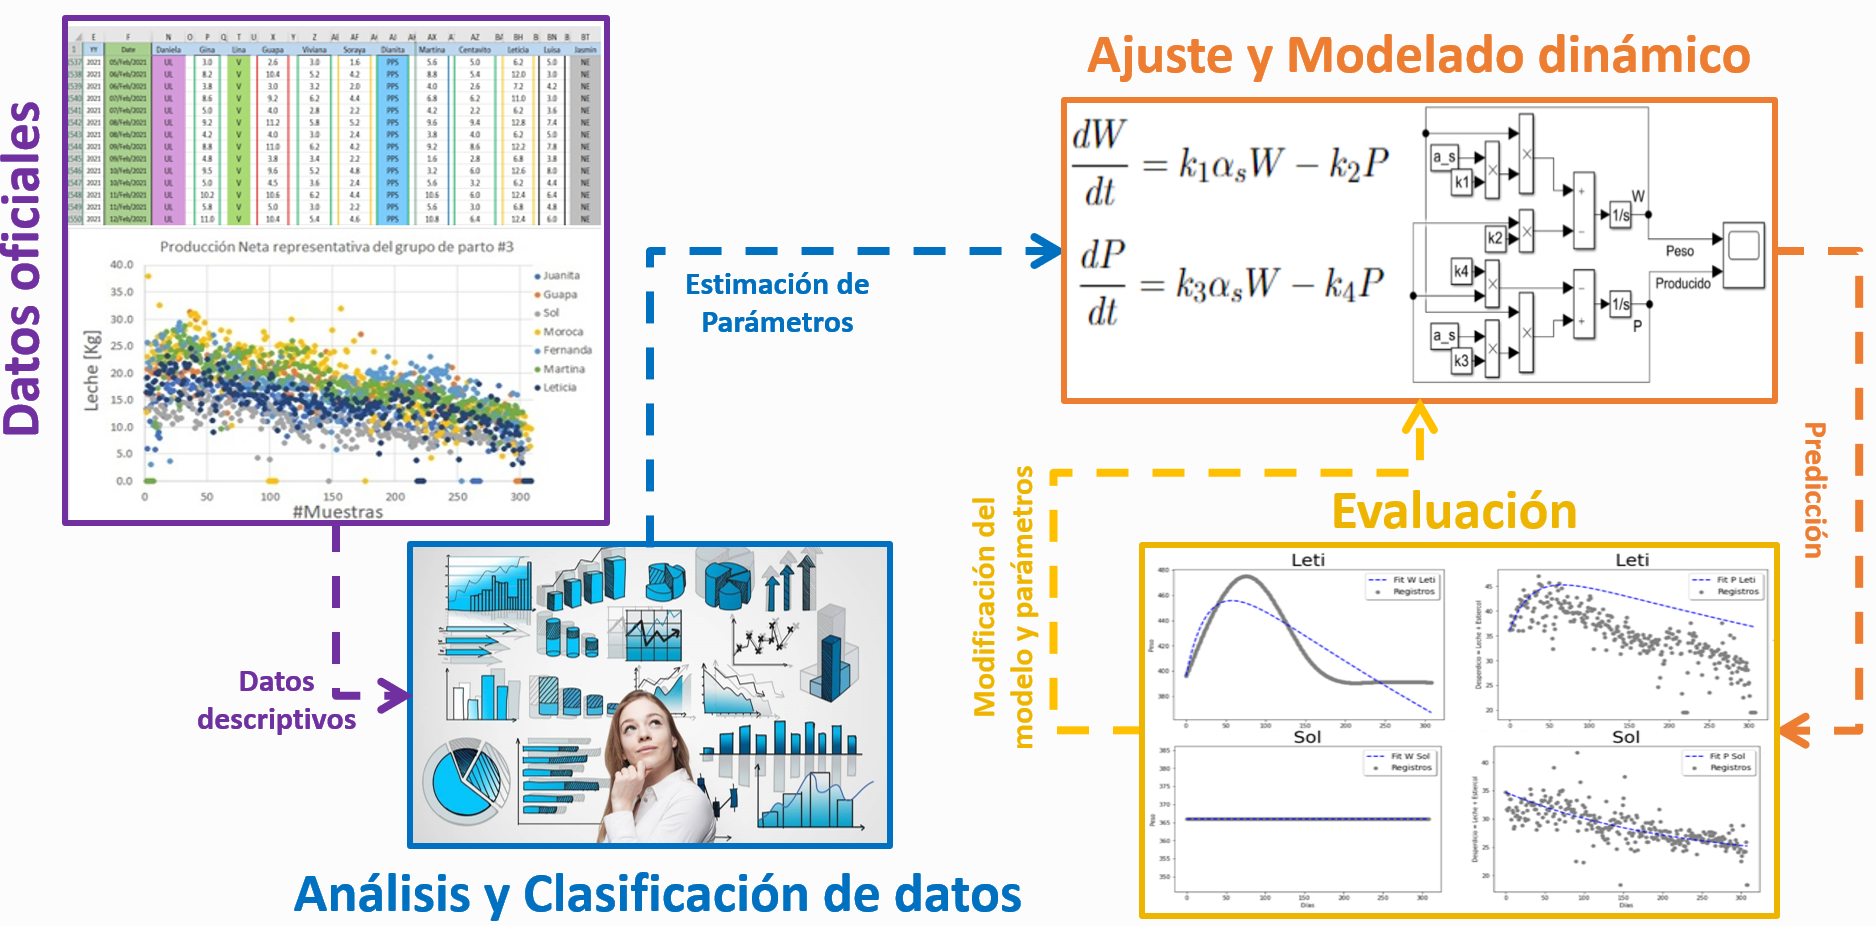
\includegraphics[width=\textwidth]{img/tesispptsena.png}
    \caption{Planteamiento general de las etapas 2, 3, 4 y 5 de la metodología usada en la ejecución del proyecto.}
    \label{tesispptsenapng}
\end{figure}

Es importante considerar este diagrama de bloques cómo una guía para comprender el plan de acción llevado a lo largo de éste proyecto de investigación. No obstante, cada una de las etapas previamente mencionadas estarán explicadas en mayor detalle a lo largo del desglose de las etapas de la metodología CRISP-DM de Entendimiento de los datos (ver Capítulo \ref{crisp2}), Preparación de los datos (ver Capítulo \ref{crisp3}), Modelación (ver Capítulo \ref{crisp4}) y Evaluación (ver Capítulo \ref{crisp5}).



\pagebreak

